%        File: arfc-beamer.tex
%     Created: Sun May 5 10:00 PM 2013 C
%


%\documentclass[11pt,handout]{beamer}
\documentclass[9pt]{beamer}
\usetheme[white]{Illinois}
%\title[short title]{long title}
\title[Short Title]{Dynamic Transition Analysis with TIMES}
%\subtitle[short subtitle]{long subtitle}
%\subtitle[Short SubTitle]{Mostly Kittens}
%\author[short name]{long name}
\author[Anshuman Chaube]{Anshuman Chaube, Andrew Chapman, James Stubbins, Kathryn Huff}
%\date[short date]{long date}
\date[01.02.2019]{February 1, 2019 \\ I$^2$CNER INTERNATIONAL WORKSHOP \\ ENERGY ANALYSIS DIVISION}
%\institution[short name]{long name}
\institute[UIUC]{University of Illinois at Urbana-Champaign \\ International Institute for Carbon-Neutral Energy Research}
%\institute[I2CNER]{International Institute for Carbon-Neutral Energy Research}

%\usepackage{bbding}
\usepackage{amsfonts}
\usepackage{amsmath}
\usepackage{xspace}
\usepackage{graphicx}
\usepackage{subfigure}
\usepackage{booktabs} % nice rules for tables
\usepackage{microtype} % if using PDF
\usepackage{bigints}
%\usepackage{minted}

\newcommand{\units}[1] {\:\text{#1}}%
\newcommand{\SN}{S$_N$}%{S$_\text{N}$}%{$S_N$}%
\DeclareMathOperator{\erf}{erf}
%I need some complimentary error funcitons... 
\DeclareMathOperator{\erfc}{erfc}
%page numbers
\setbeamertemplate{footline}[page number]
\setbeamertemplate{caption}[numbered]
%Those icons in the references are terrible looking
\setbeamertemplate{bibliography item}[text]

% ------------CHECK MARKS -------------------------
\usepackage{amssymb}
\usepackage{pifont}
\usepackage{xcolor}
\newcommand{\greencheck}{{\color{green}\checkmark}}
\newcommand{\xmark}{{\color{red}\ding{55}}}
%--------------------------------------------------

%---------------TIKZ-------------------------------
\usepackage{tikz}
\usepackage{scalefnt}
\usepackage{chronology}
\usetikzlibrary{arrows.meta}

\usetikzlibrary{positioning, arrows, decorations, shapes, calc }
% Define block styles

\usetikzlibrary{shapes.multipart}
\usetikzlibrary{positioning}
\usetikzlibrary{backgrounds,scopes} 
%--------------------------------------------------

%%%% Acronym support

\usepackage[acronym,toc]{glossaries}
\newacronym{<++>}{<++>}{<++>}
\newacronym{I$^2$CNER}{I$^2$CNER}{International Institute for Carbon Neutral Energy Research}
\newacronym{MARKAL}{MARKAL}{MARKet ALlocation}
\newacronym{TIMES}{TIMES}{The Integrated MARKAL-EFOM System}
%\newacronym[longplural={metric tons of heavy metal}]{MTHM}{MTHM}{metric ton of heavy metal}



\makeglossaries

%try to get rid of header on title page\dots
\makeatletter
    \newenvironment{withoutheadline}{
        \setbeamertemplate{headline}[default]
        \def\beamer@entrycode{\vspace*{-\headheight}}
    }{}
\makeatother

\begin{document}
%%%%%%%%%%%%%%%%%%%%%%%%%%%%%%%%%%%%%%%%%%%%%%%%%%%%%%%%%%%%%
%% From uw-beamer Here's a handy bit of code to place at 
%% the beginning of your presentation (after \begin{document}):
\newcommand*{\alphabet}{ABCDEFGHIJKLMNOPQRSTUVWXYZabcdefghijklmnopqrstuvwxyz}
\newlength{\highlightheight}
\newlength{\highlightdepth}
\newlength{\highlightmargin}
\setlength{\highlightmargin}{2pt}
\settoheight{\highlightheight}{\alphabet}
\settodepth{\highlightdepth}{\alphabet}
\addtolength{\highlightheight}{\highlightmargin}
\addtolength{\highlightdepth}{\highlightmargin}
\addtolength{\highlightheight}{\highlightdepth}
\newcommand*{\Highlight}{\rlap{\textcolor{HighlightBackground}{\rule[-\highlightdepth]{\linewidth}{\highlightheight}}}}
%%%%%%%%%%%%%%%%%%%%%%%%%%%%%%%%%%%%%%%%%%%%%%%%%%%%%%%%%%%%%
%%--------------------------------%%
\begin{withoutheadline}
\frame{
  \titlepage
}
\end{withoutheadline}

%%--------------------------------%%
\AtBeginSection[]{
\begin{frame}
  \frametitle{Outline}
  \tableofcontents[currentsection]
\end{frame}
}

\section{Motivation}
%\subsection{Cat Behavior}
%\begin{frame}
  %\frametitle{Motivation}
  % a comment
%  \begin{figure}[htbp!]
%    \begin{center}
%      
\includegraphics[height=4cm]{./images/kitten}
%    \end{center}
%          \caption{A caption describing the image. \cite{lastname_firstword_1900}.}
%    \label{fig:kittenfigure}
%  \end{figure}
%\end{frame}

\begin{frame}
  \frametitle{Motivation}
   \begin{itemize}
   
   \item Dynamic transition analysis to minimize CO$_2$ emissions in Japan.
   
   \item Focus on optimizing \textbf{electricity supply}.
   
   \item \textbf{I$^2$CNER goal:} Reduce emissions by 80\% from 1990 levels by 2050. 
   
   \item After 2050: emissions held constant until 2100 if possible.
   
   \item Energy supply includes conventional and some I$^2$CNER technology.
   
   \item Using The Integrated MARKAL-EFOM System (TIMES) \cite{loulou_documentation_2005}.
   \end{itemize}
        
\end{frame}

%\subsection{Cat Appearance}
%\begin{frame}
  \frametitle{Columns}
  % a comment
        \begin{columns}
                \column[t]{5cm}
                Sometimes things need to be put side by side, in two nice 
                looking columns. 

                Maybe one column involves a quotation.

                \begin{quote}
                        Explicit is better than implicit. -- The Zen of Python
                \end{quote}


                And, also, perhaps, a logo.
                \begin{center}
                        
\includegraphics[height=0.2\textheight]{./images/arfc-logo}
                \end{center}
                \column[t]{5cm}
        \begin{figure}[htbp!]
        \begin{center}
      
\includegraphics[height=4cm]{./images/kitten}
    \end{center}
          \caption{A caption describing the image. \cite{lastname_firstword_1900}.}
    \label{fig:kittenfigure}
  \end{figure}
        \end{columns}
\end{frame}

\begin{frame}[fragile]
  \frametitle{Some Code}
        I have to use the fragile syntax for code slides.
        \begin{minted}{python}
def meow(volume):
    """Make a demanding noise at the specified volume
    
    Parameters
    ----------
    volume: int
        The volume of the demand. No relation to importance.

    Returns
    -------
    str
        meow
    """
    o = 'o'*volume
    return 'me'+ o + 'ow'
\end{minted}
\end{frame}

%\subsection{Cat Math}
%\begin{frame}
  \frametitle{Cat Math: Part 1}
  % a comment
        \begin{align}
                x &= y
                \intertext{where}
                x &= \mbox{cats}\\
                y &= \mbox{peculiar}
        \end{align}
\end{frame}

\begin{frame}
\frametitle{Cat Math: Part 2}
        Everything in Beamer is just like in \LaTeX.
        Right down to the theorems.
        \begin{theorem}[Pythagoras] 
                $ a^2 + b^2 = c^2$
        \end{theorem}
        \begin{corollary}
                $ x + y = y + x  $
        \end{corollary}
        \begin{proof}
                $\omega +\phi = \epsilon $
        \end{proof}


\end{frame}

\section{Methodology}
\subsection{Basics}
\begin{frame}
  \frametitle{Basics}
  % a comment
        \begin{itemize}
        
        \item Constrained linear/mixed-linear optimization problem.
        
        \item Objective function - System Cost.
        
        \item Constraints - CO$_2$ emissions, demand.
        
        \item Novel tech - H$_2$ (steam reforming, photocatalytic conversion), carbon capture and sequestration (absorption type).
        
        \end{itemize}
\end{frame}

\subsection{Assumptions}
\begin{frame}
  \frametitle{Assumptions}

  \begin{itemize}
  
  \item New Nuclear = ABWRs
  
  \item Nuclear, wind, solar growth rates based on trends in USA, China, Japan.
  
  \item CCS: Available for deployment in 2030, costs reduce by 2050.
  
  \item H$_2$: Steam reforming available in 2030, photocatalytic conversion in 2050.
  
  \item Hydropower, geothermal capacity held constant.
  
  \end{itemize}

\end{frame}

\subsection{Limitations}
\begin{frame}
  \frametitle{Limitations}
  % a comment
        \begin{itemize}
        
         \item Focus entirely on \textbf{electricity supply sector}.      
         
         \item Cost of fossil fuels, geothermal, hydropower, steam reforming and nuclear is constant.
         
         \item Area cost not taken into account.
         
         \item Emissions tied to energy production, not capacity installation.
         
         \item Annual time-step cannot capture seasonal/daily variation in wind, solar (however annually averaged availability factors are incorporated).
        
        \end{itemize}

\end{frame}

\subsection{Scenarios}
\begin{frame}
  \frametitle{Scenarios}
  % a comment
\begin{tabular}{| c | c | c | c | c |}
\hline
\textbf{Scenario}& \textbf{Figures}&\textbf{Conventional}&\textbf{I$^2$CNER}&\textbf{New nuclear}\\
                 &             &\textbf{technology}&\textbf{technology}&\textbf{reactors}\\
                  \hline
1               & Fig. \ref{s1e}\&\ref{s1c}&      \greencheck           &         \xmark       &      \greencheck     \\ 
2               & Fig. \ref{s2e}\&\ref{s2c}&      \greencheck           &         \xmark       &         \xmark       \\ 
3               & Fig. \ref{s3e}\&\ref{s3c}&      \greencheck           &      \greencheck     &      \greencheck     \\ 
4               & Fig. \ref{s4e}\&\ref{s4c}&      \greencheck           &      \greencheck     &         \xmark       \\
\hline
\end{tabular}

\end{frame}

\section{Results}
\subsection{Scenario 1}
\begin{frame}
  \frametitle{Scenario 1: No I$^2$CNER technology, with new nuclear}
  % a comment
  \begin{figure}[htbp!]
    \begin{center}
      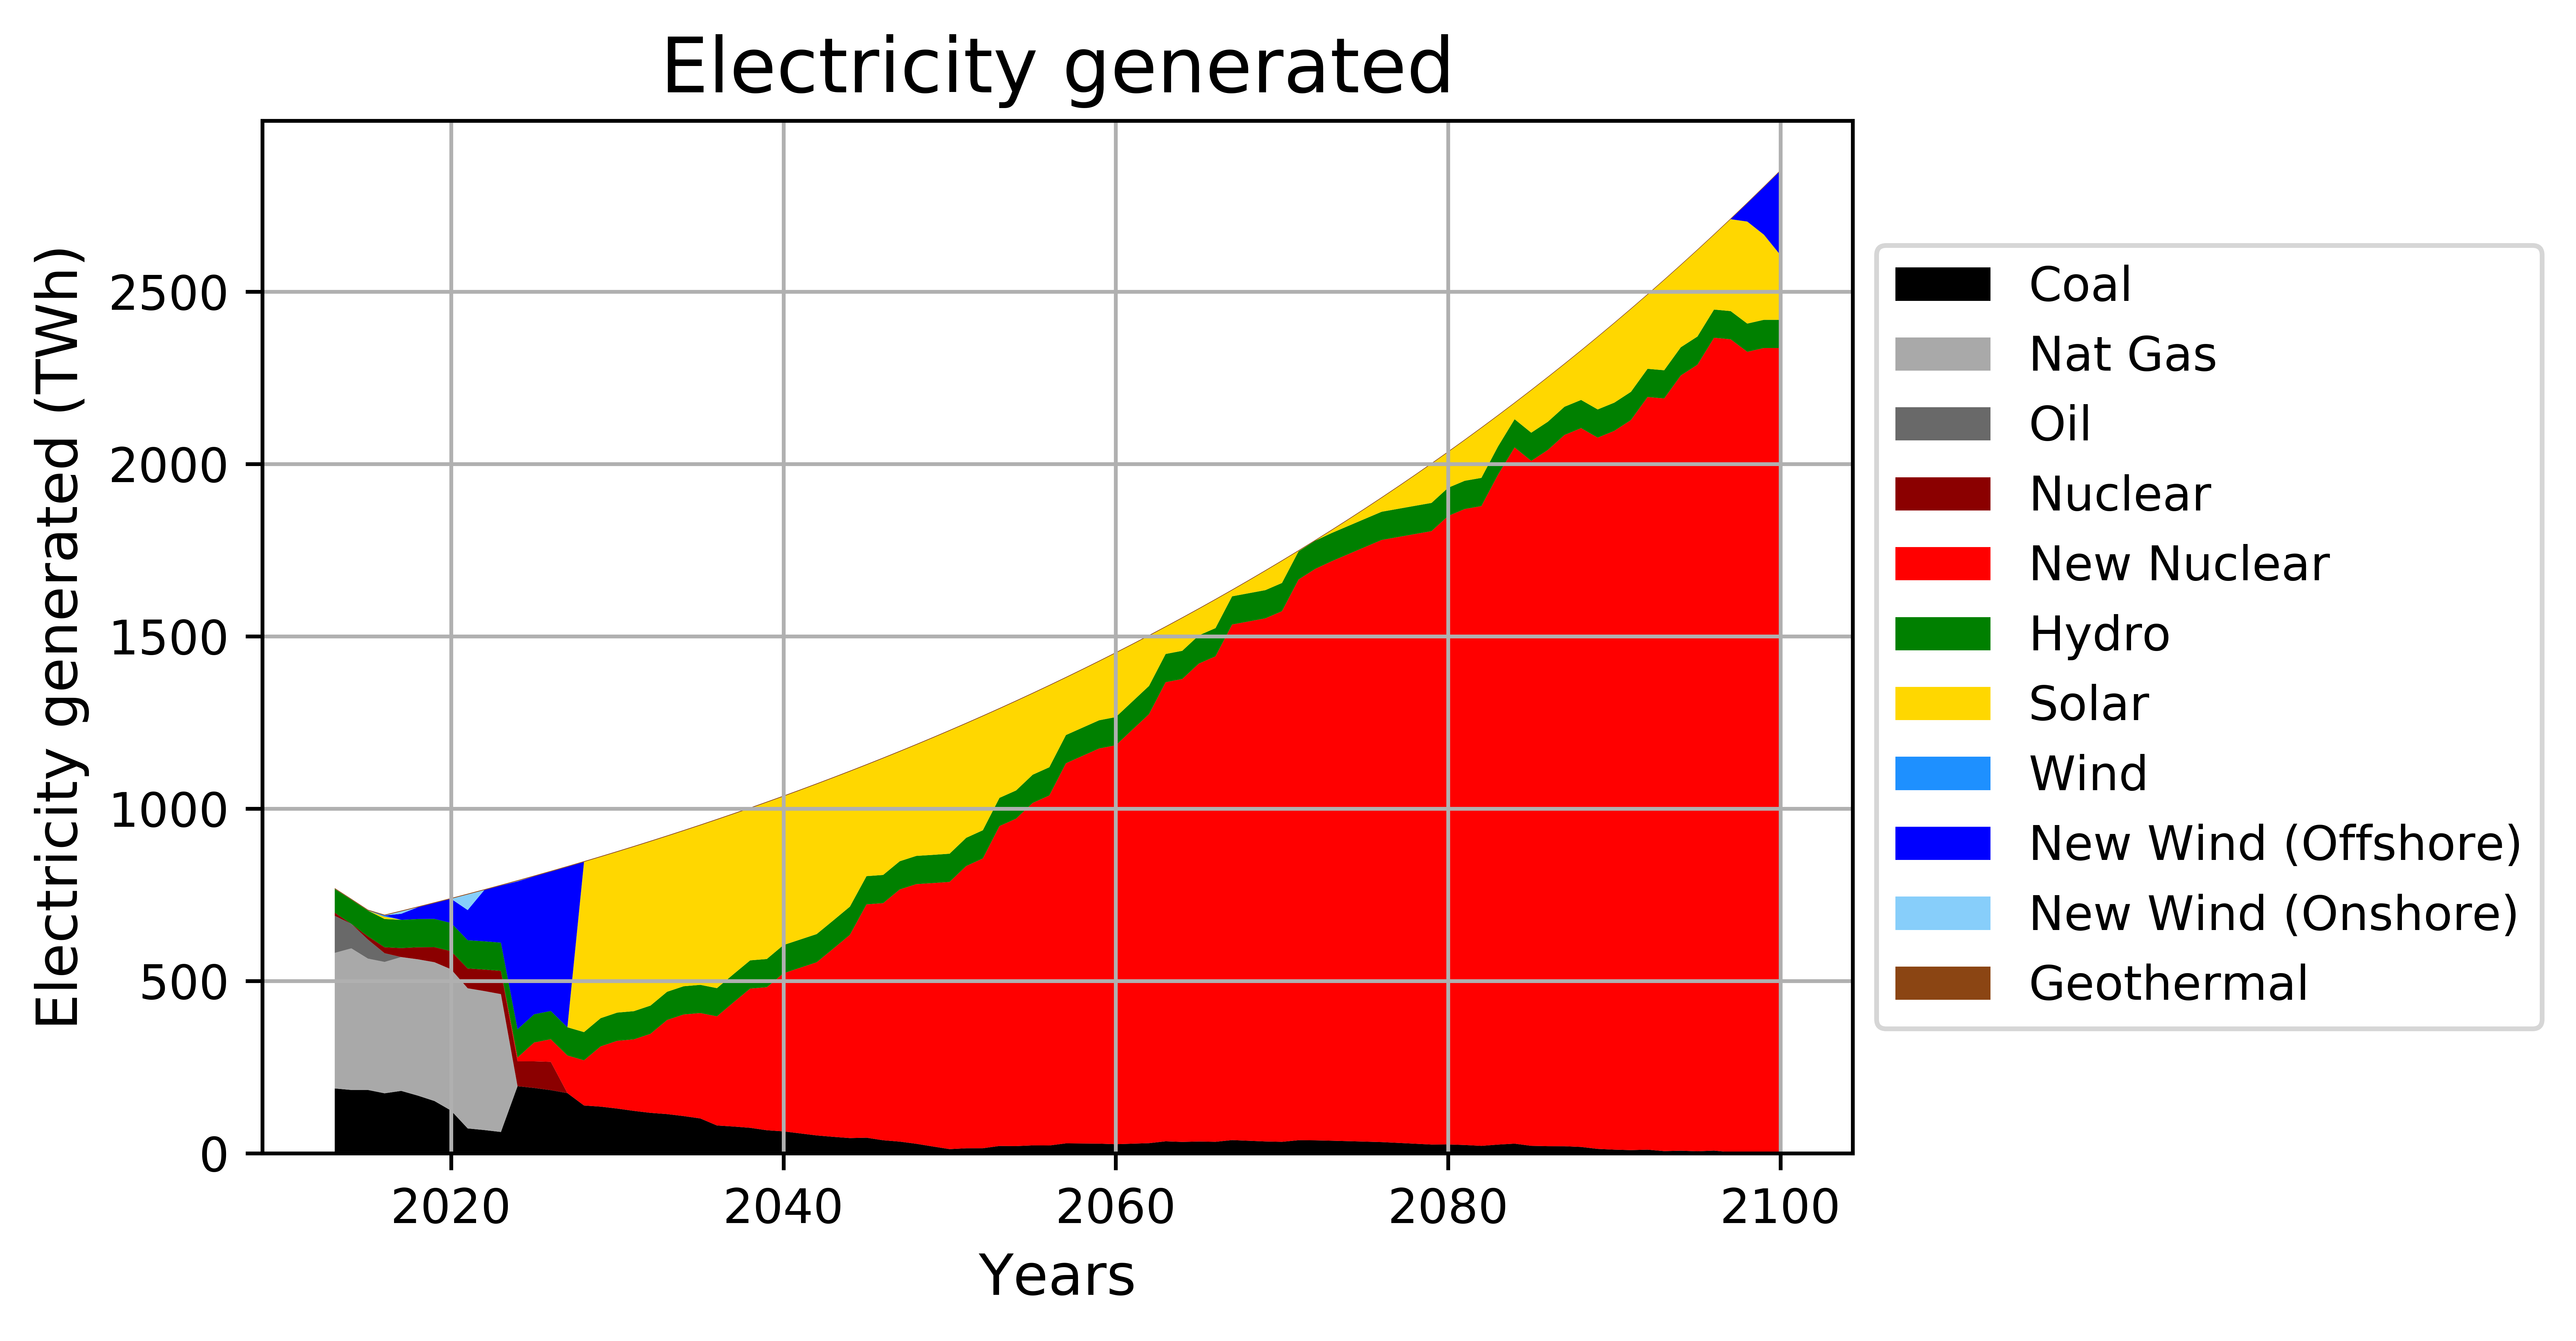
\includegraphics[scale=0.5]{./images/conv_nuc_elc}
    \end{center}
          \caption{Scenario 1 Electricity Generation.}
    \label{s1e}
  \end{figure}
\end{frame}

\begin{frame}
  \frametitle{Scenario 1: No I$^2$CNER technology, with new nuclear}
  \begin{figure}[htbp!]
    \begin{center}
      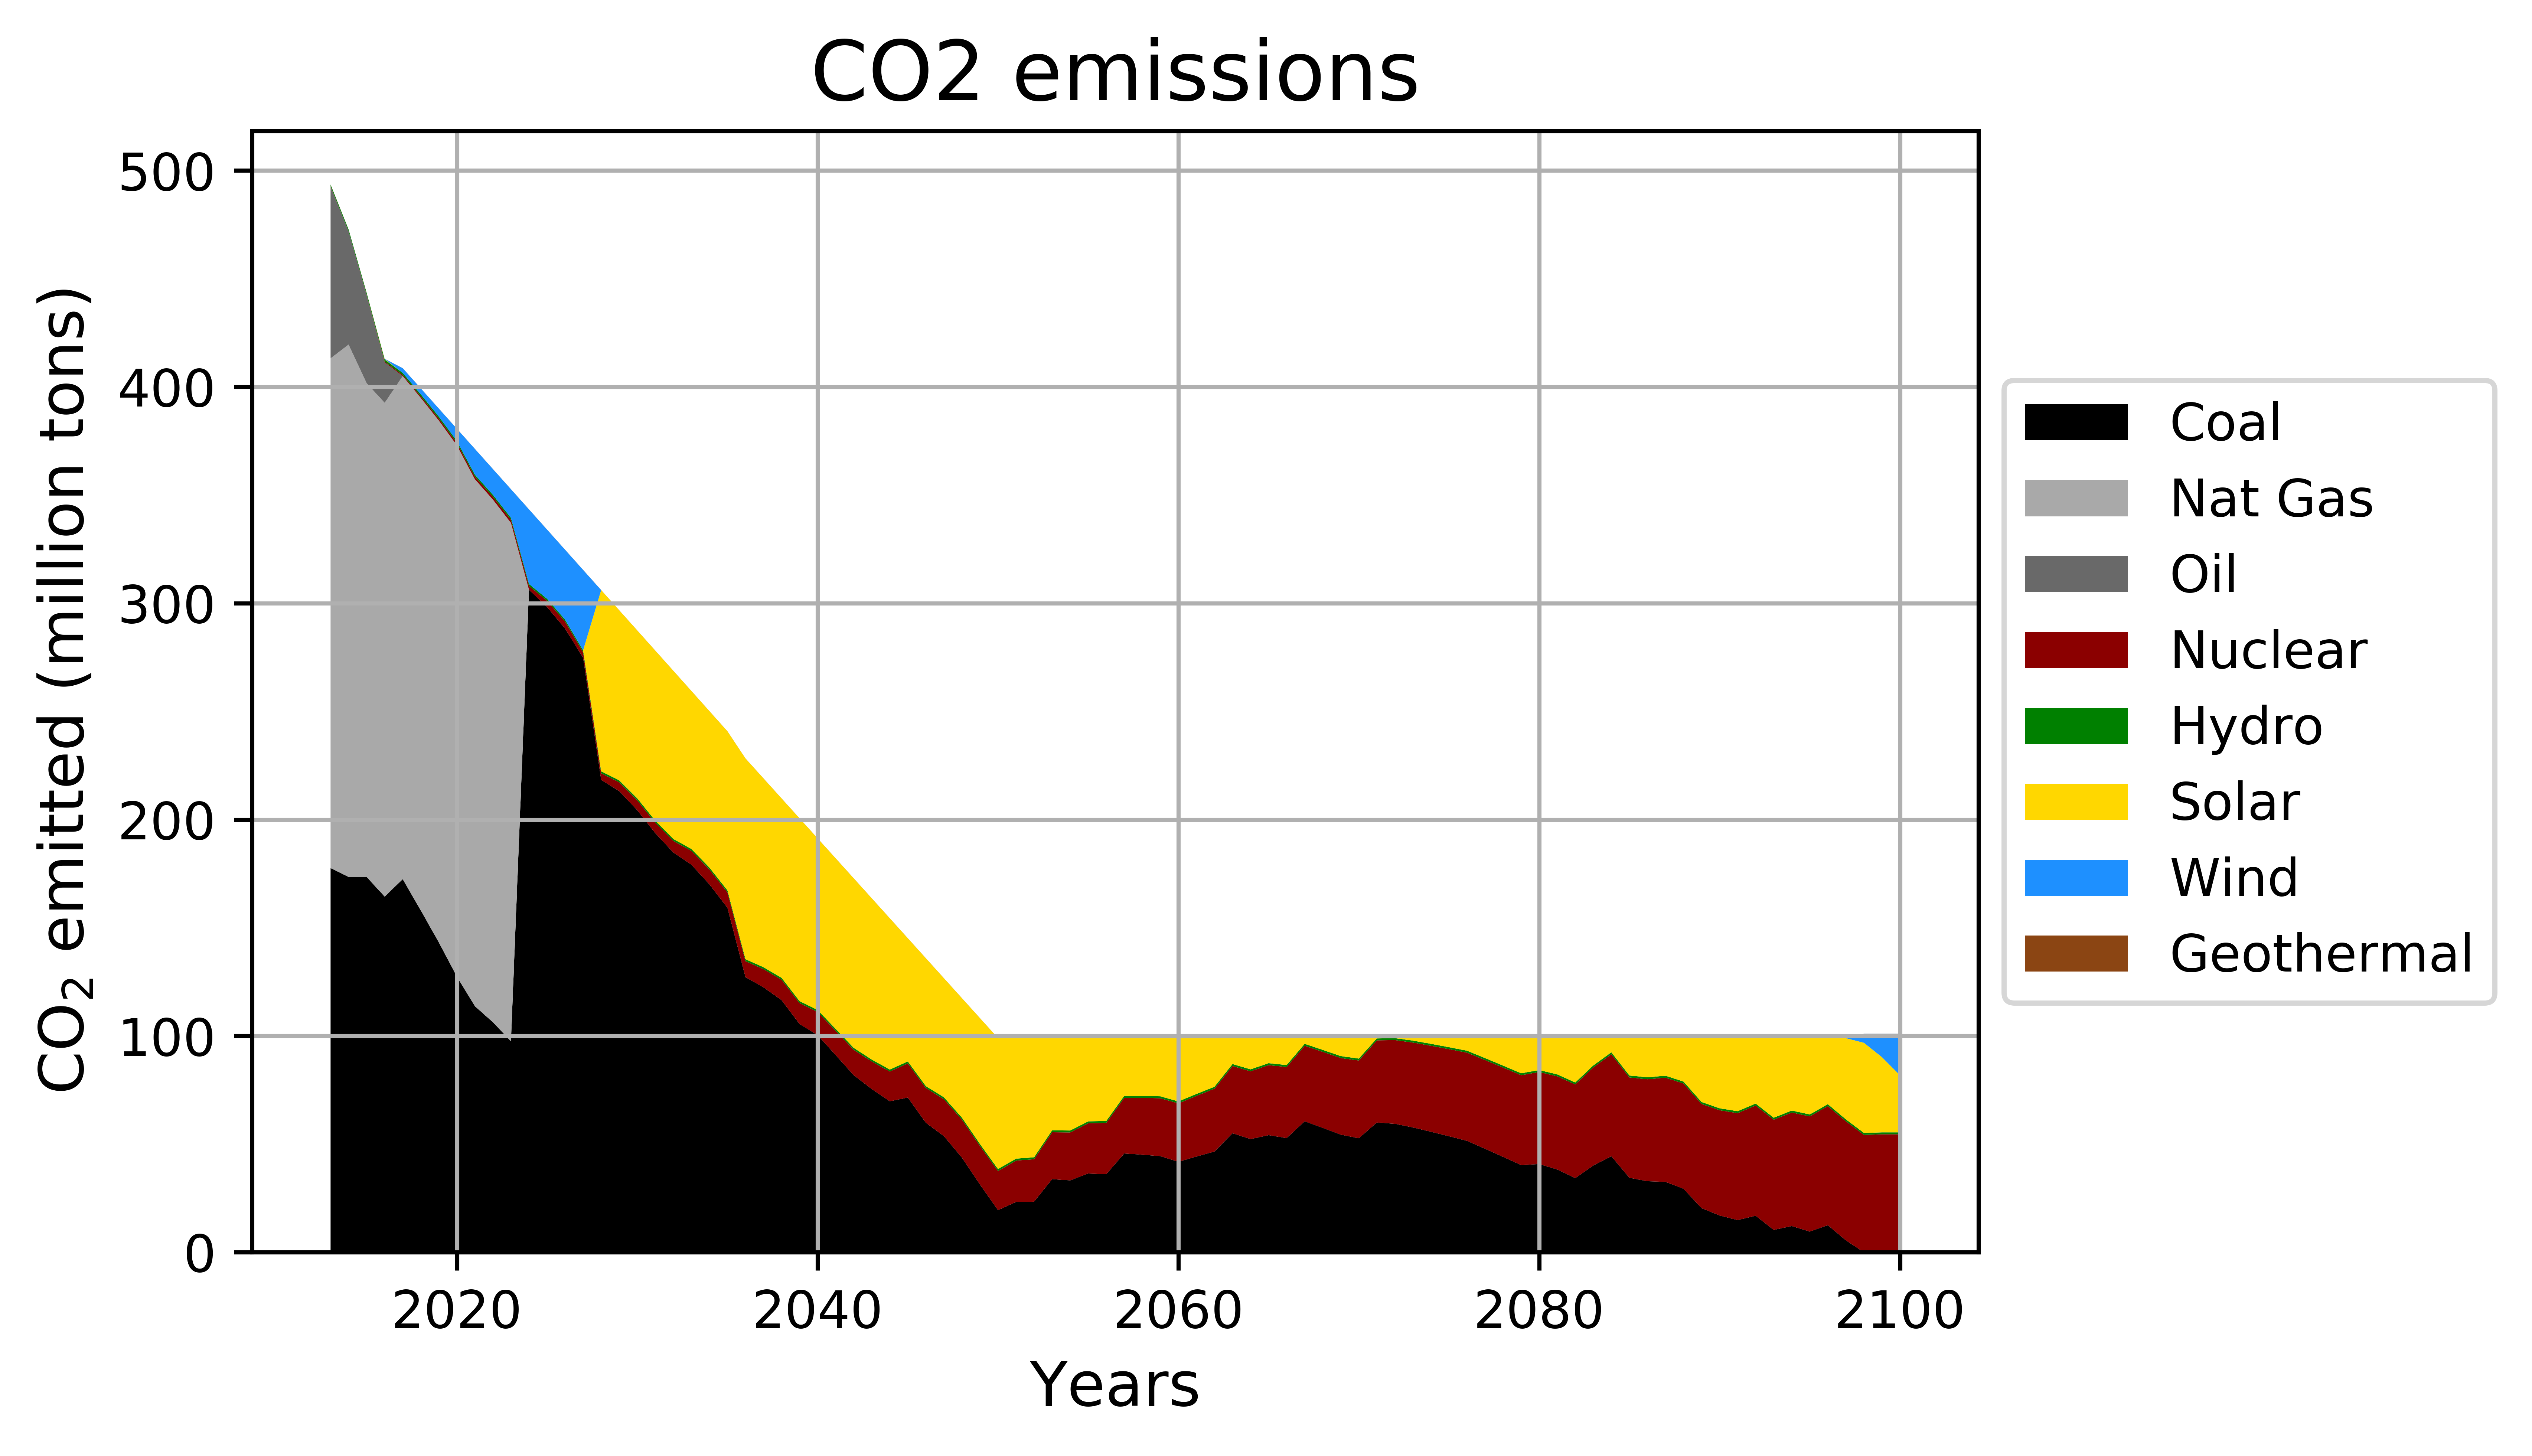
\includegraphics[scale=0.5]{./images/conv_nuc_co2}
    \end{center}
          \caption{Scenario 1 CO$_2$ emissions.}
    \label{s1c}
  \end{figure}

\end{frame}

\subsection{Scenario 2}
\begin{frame}
  \frametitle{Scenario 2}
  % a comment
  \begin{figure}[htbp!]
    \begin{center}
      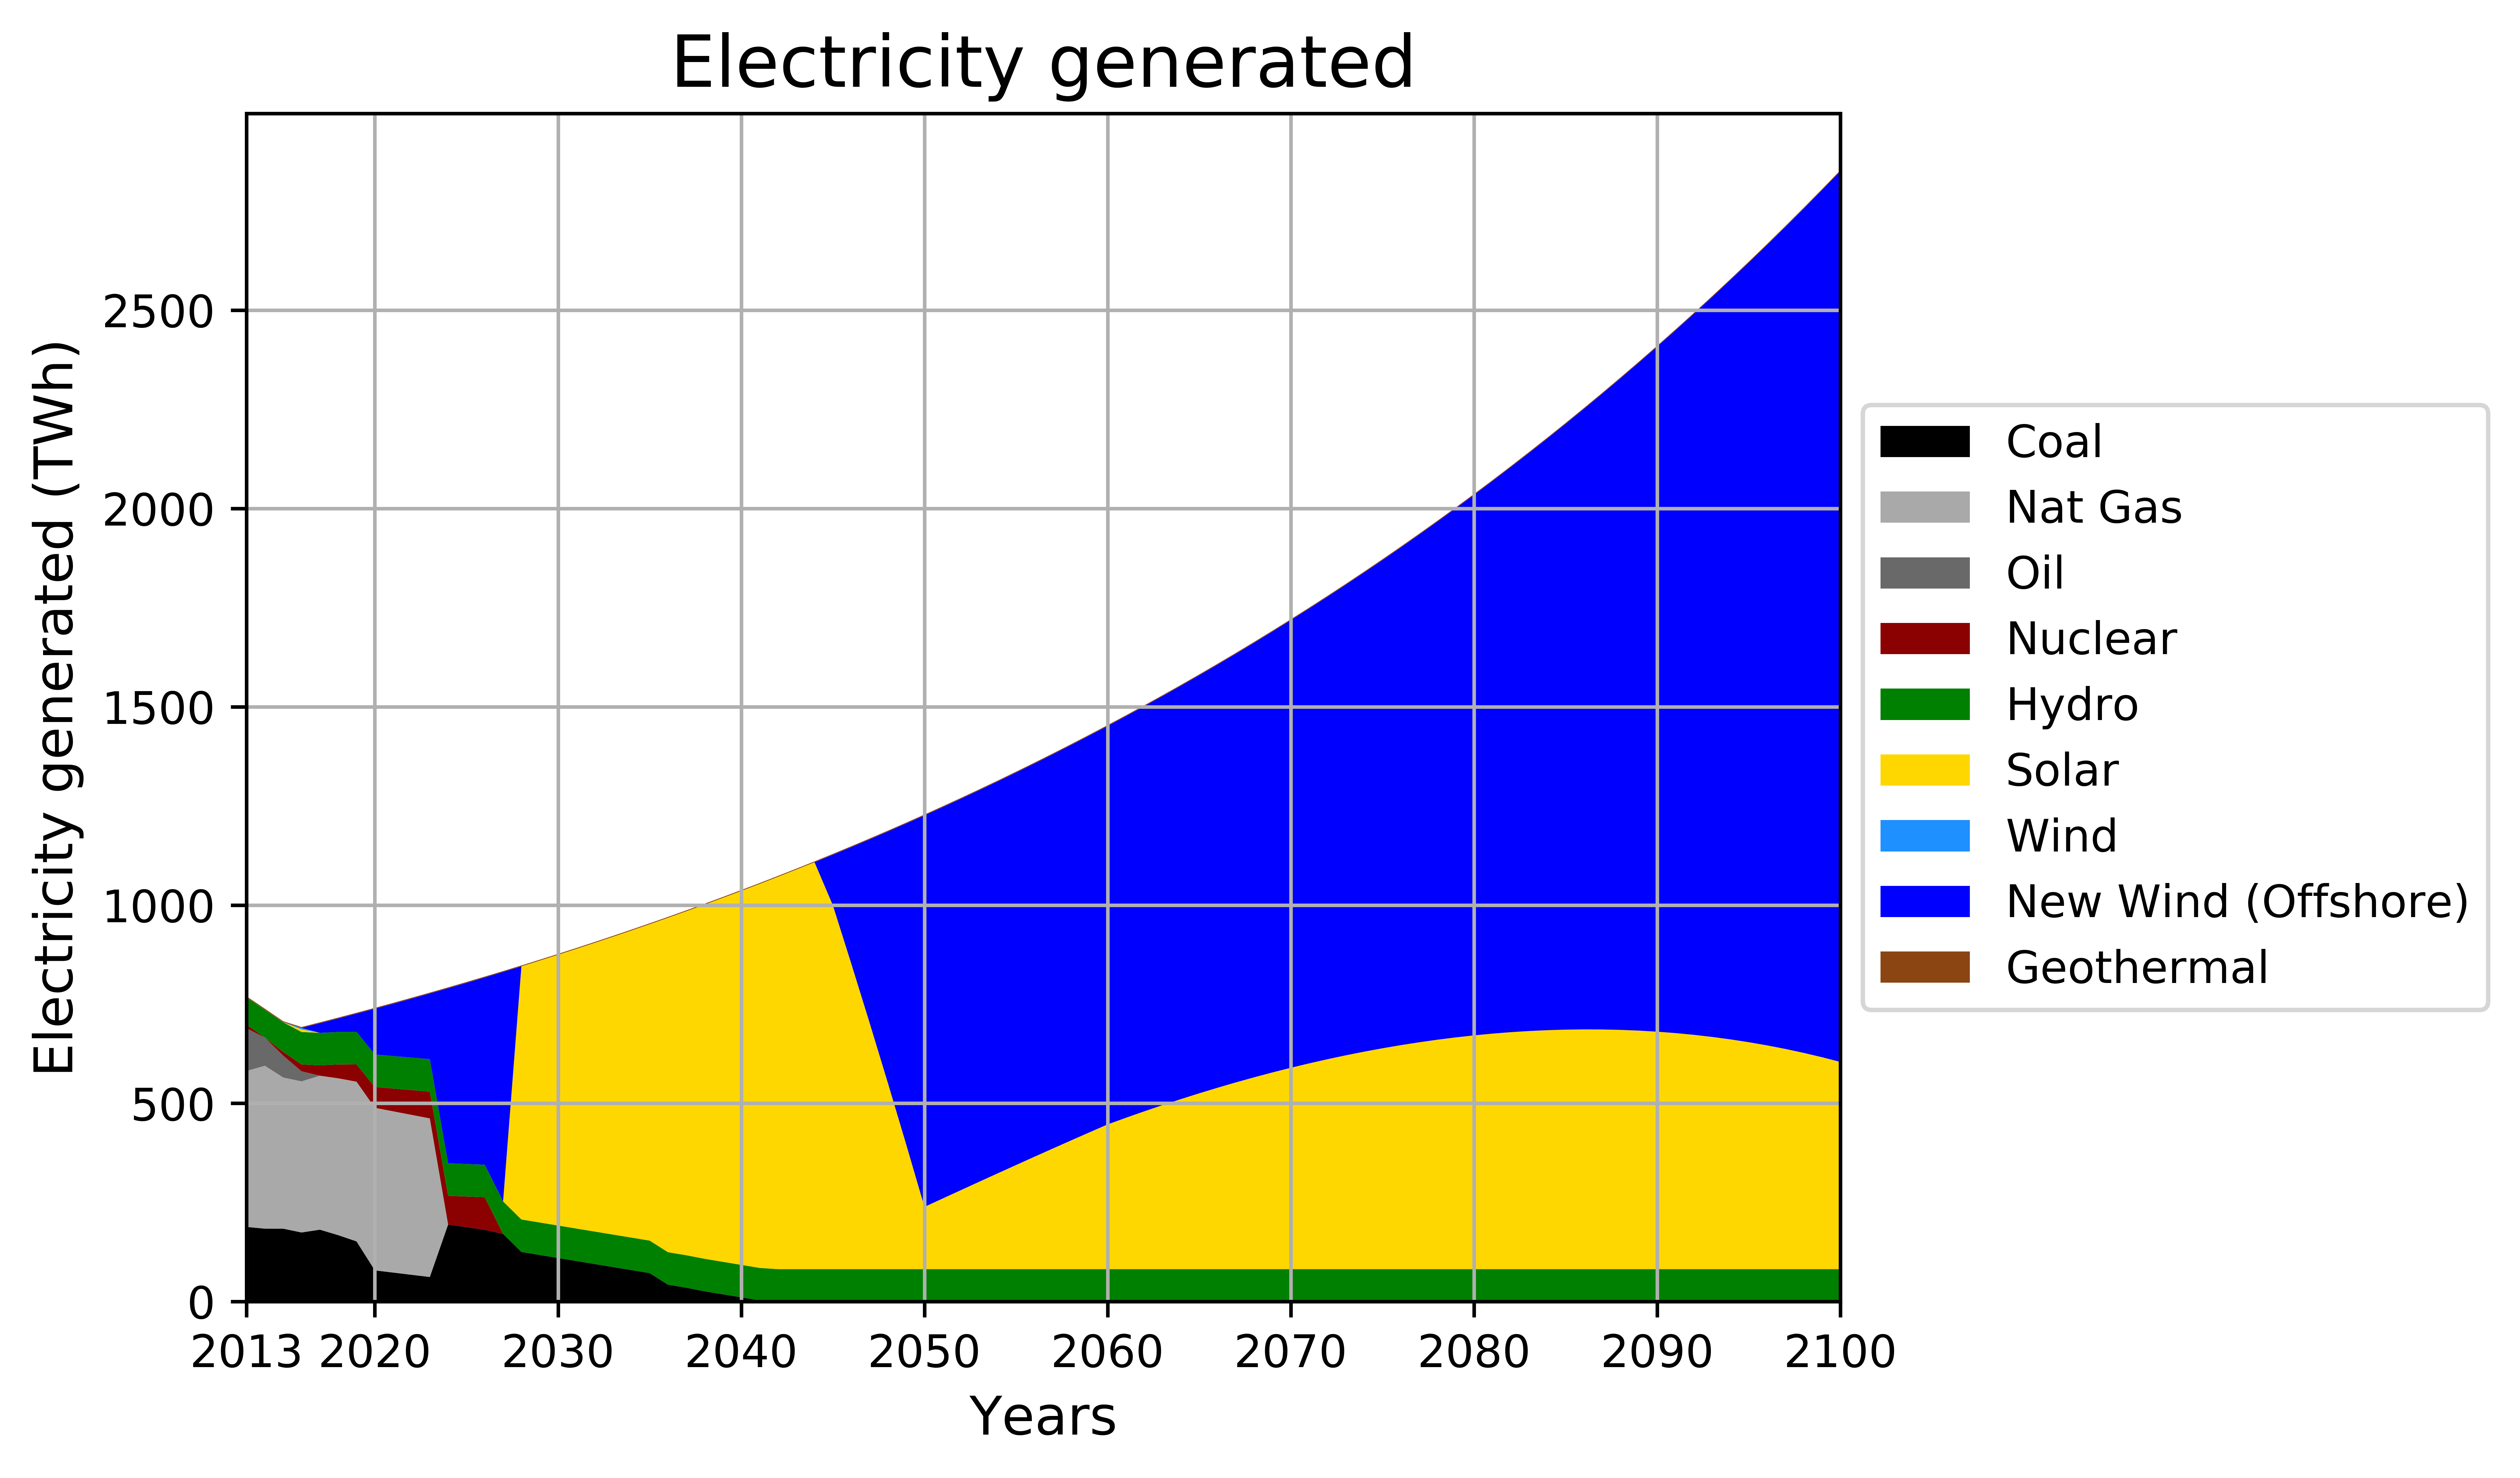
\includegraphics[scale=0.6]{./images/conv_nonuc_elc}
    \end{center}
          \caption{Scenario 2 Electricity Generation.}
    \label{s2e}
  \end{figure}
\end{frame}

\begin{frame}
  \begin{figure}[htbp!]
    \begin{center}
      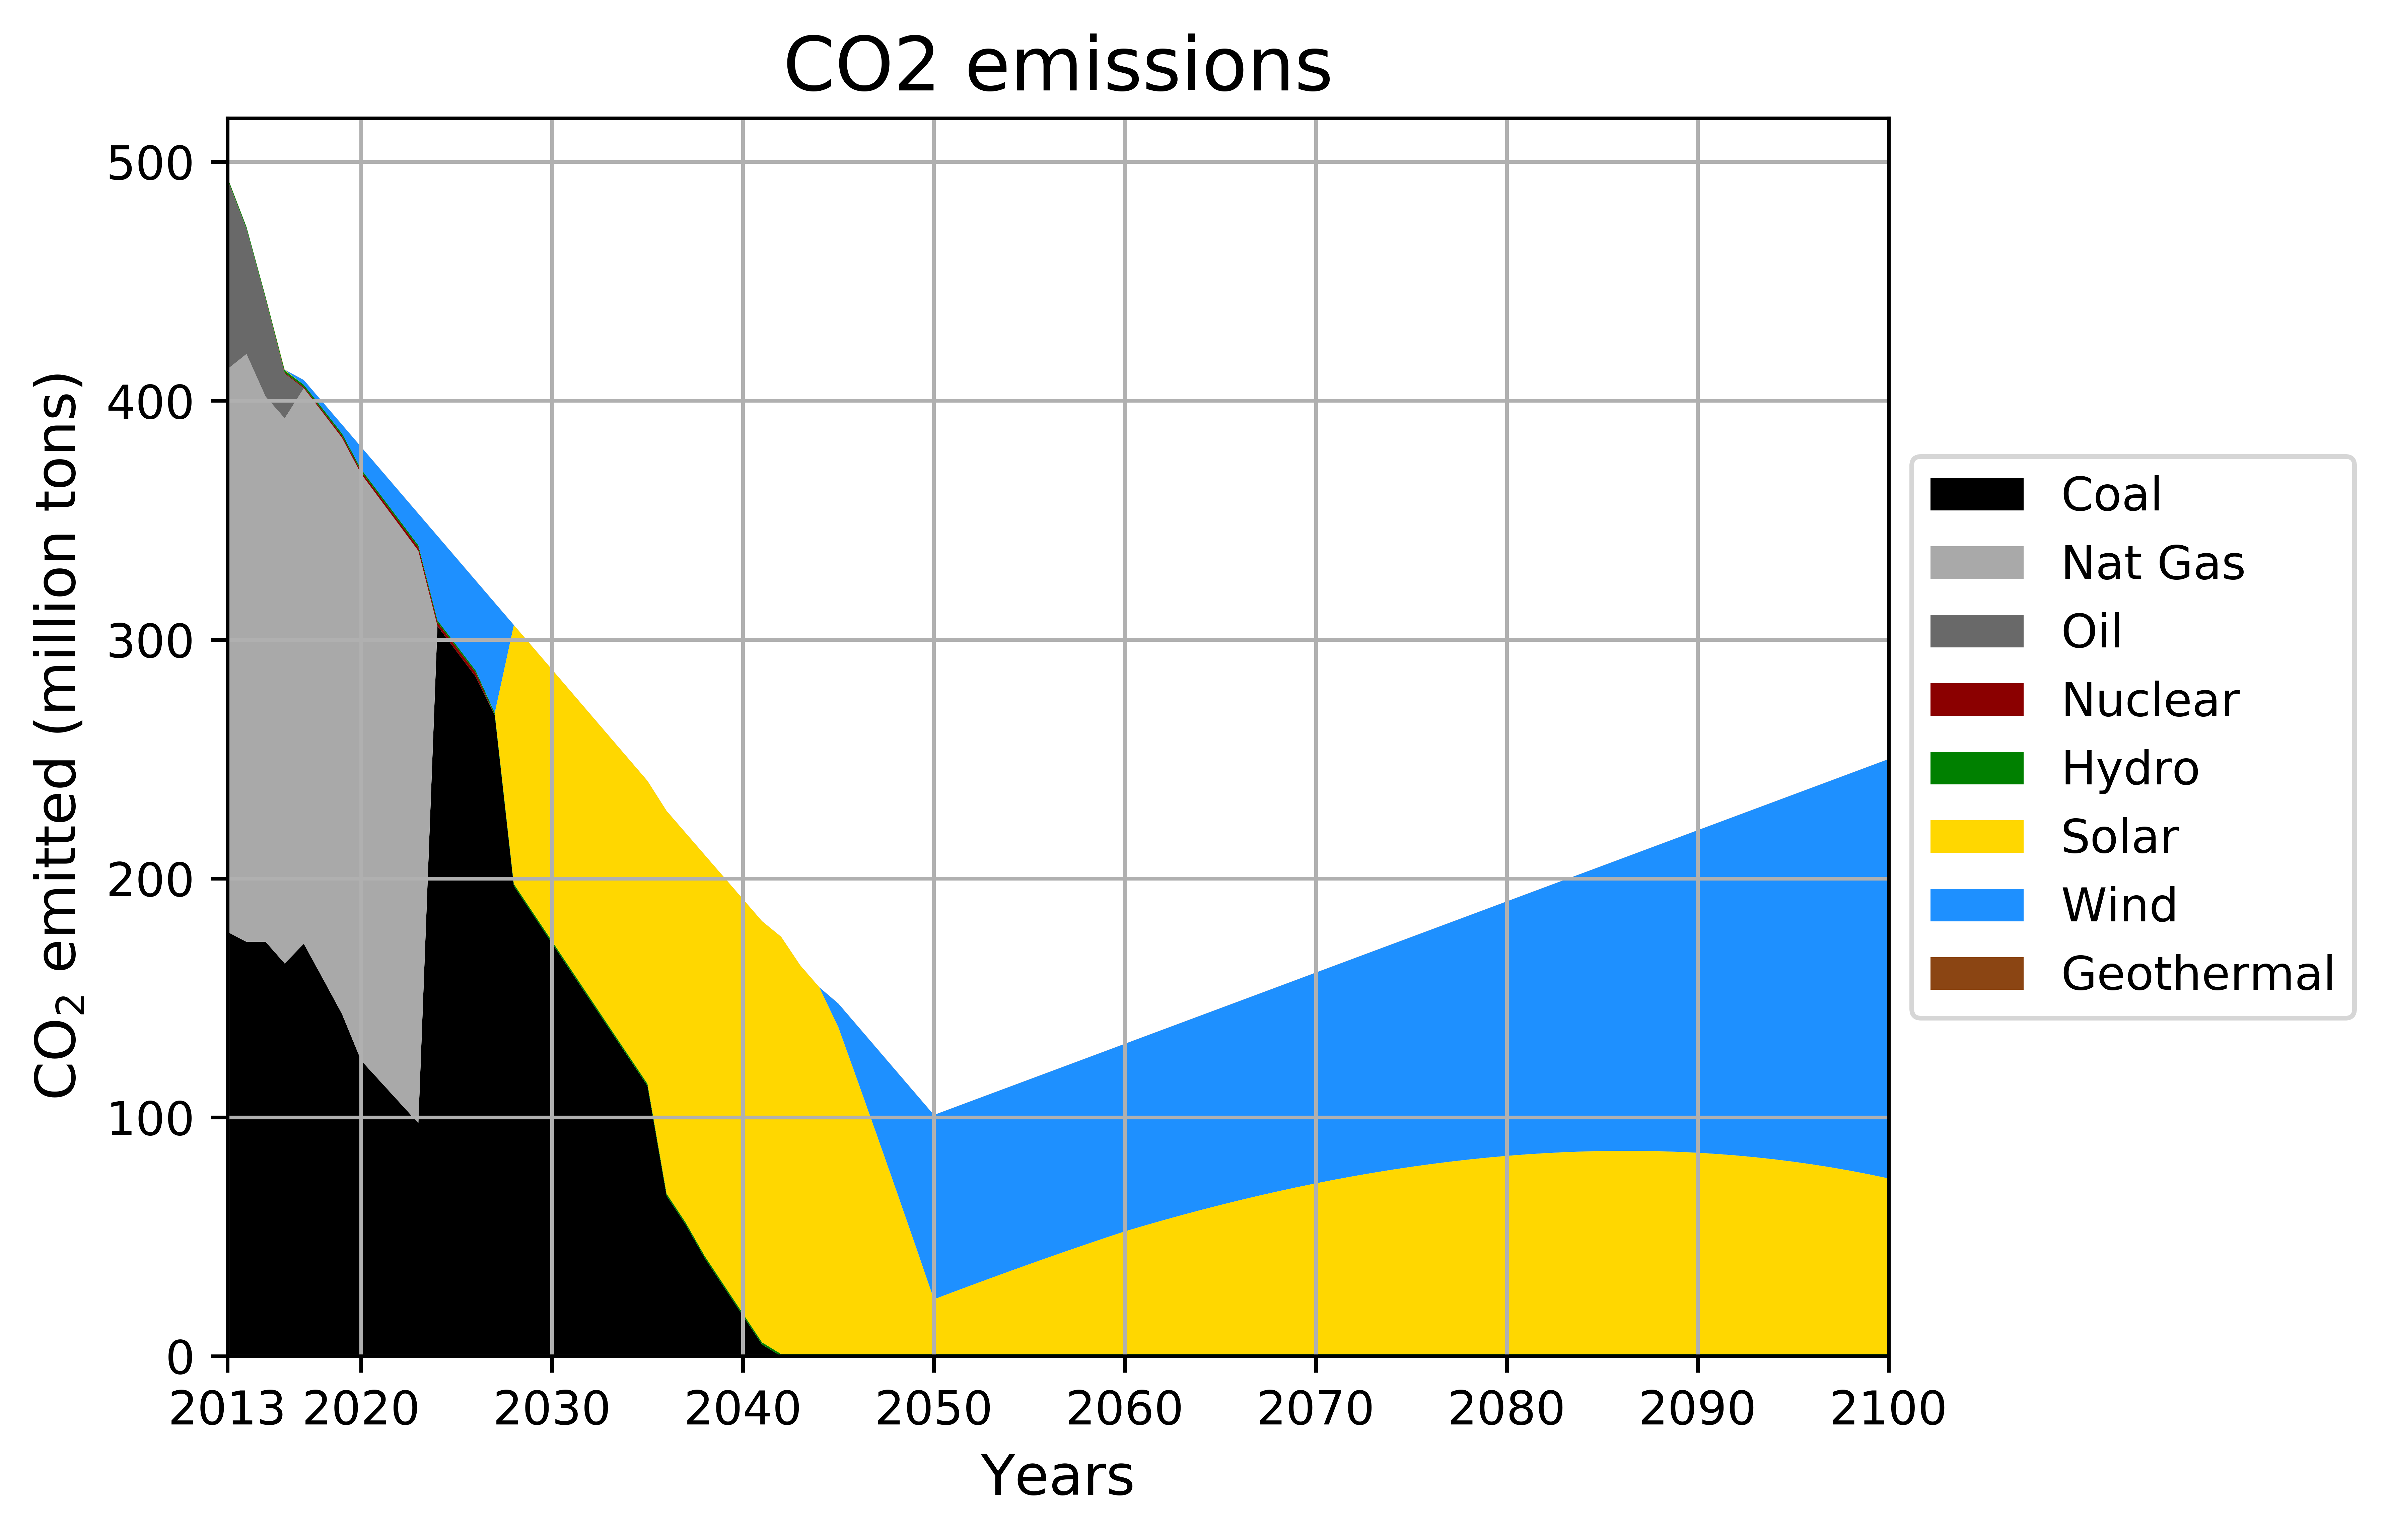
\includegraphics[scale=0.6]{./images/conv_nonuc_co2}
    \end{center}
          \caption{Scenario 2 CO$_2$ emissions.}
    \label{s2c}
  \end{figure}

\end{frame}

\subsection{Scenario 3}
\begin{frame}
  \frametitle{Scenario 3}
  % a comment
  \begin{figure}[htbp!]
    \begin{center}
      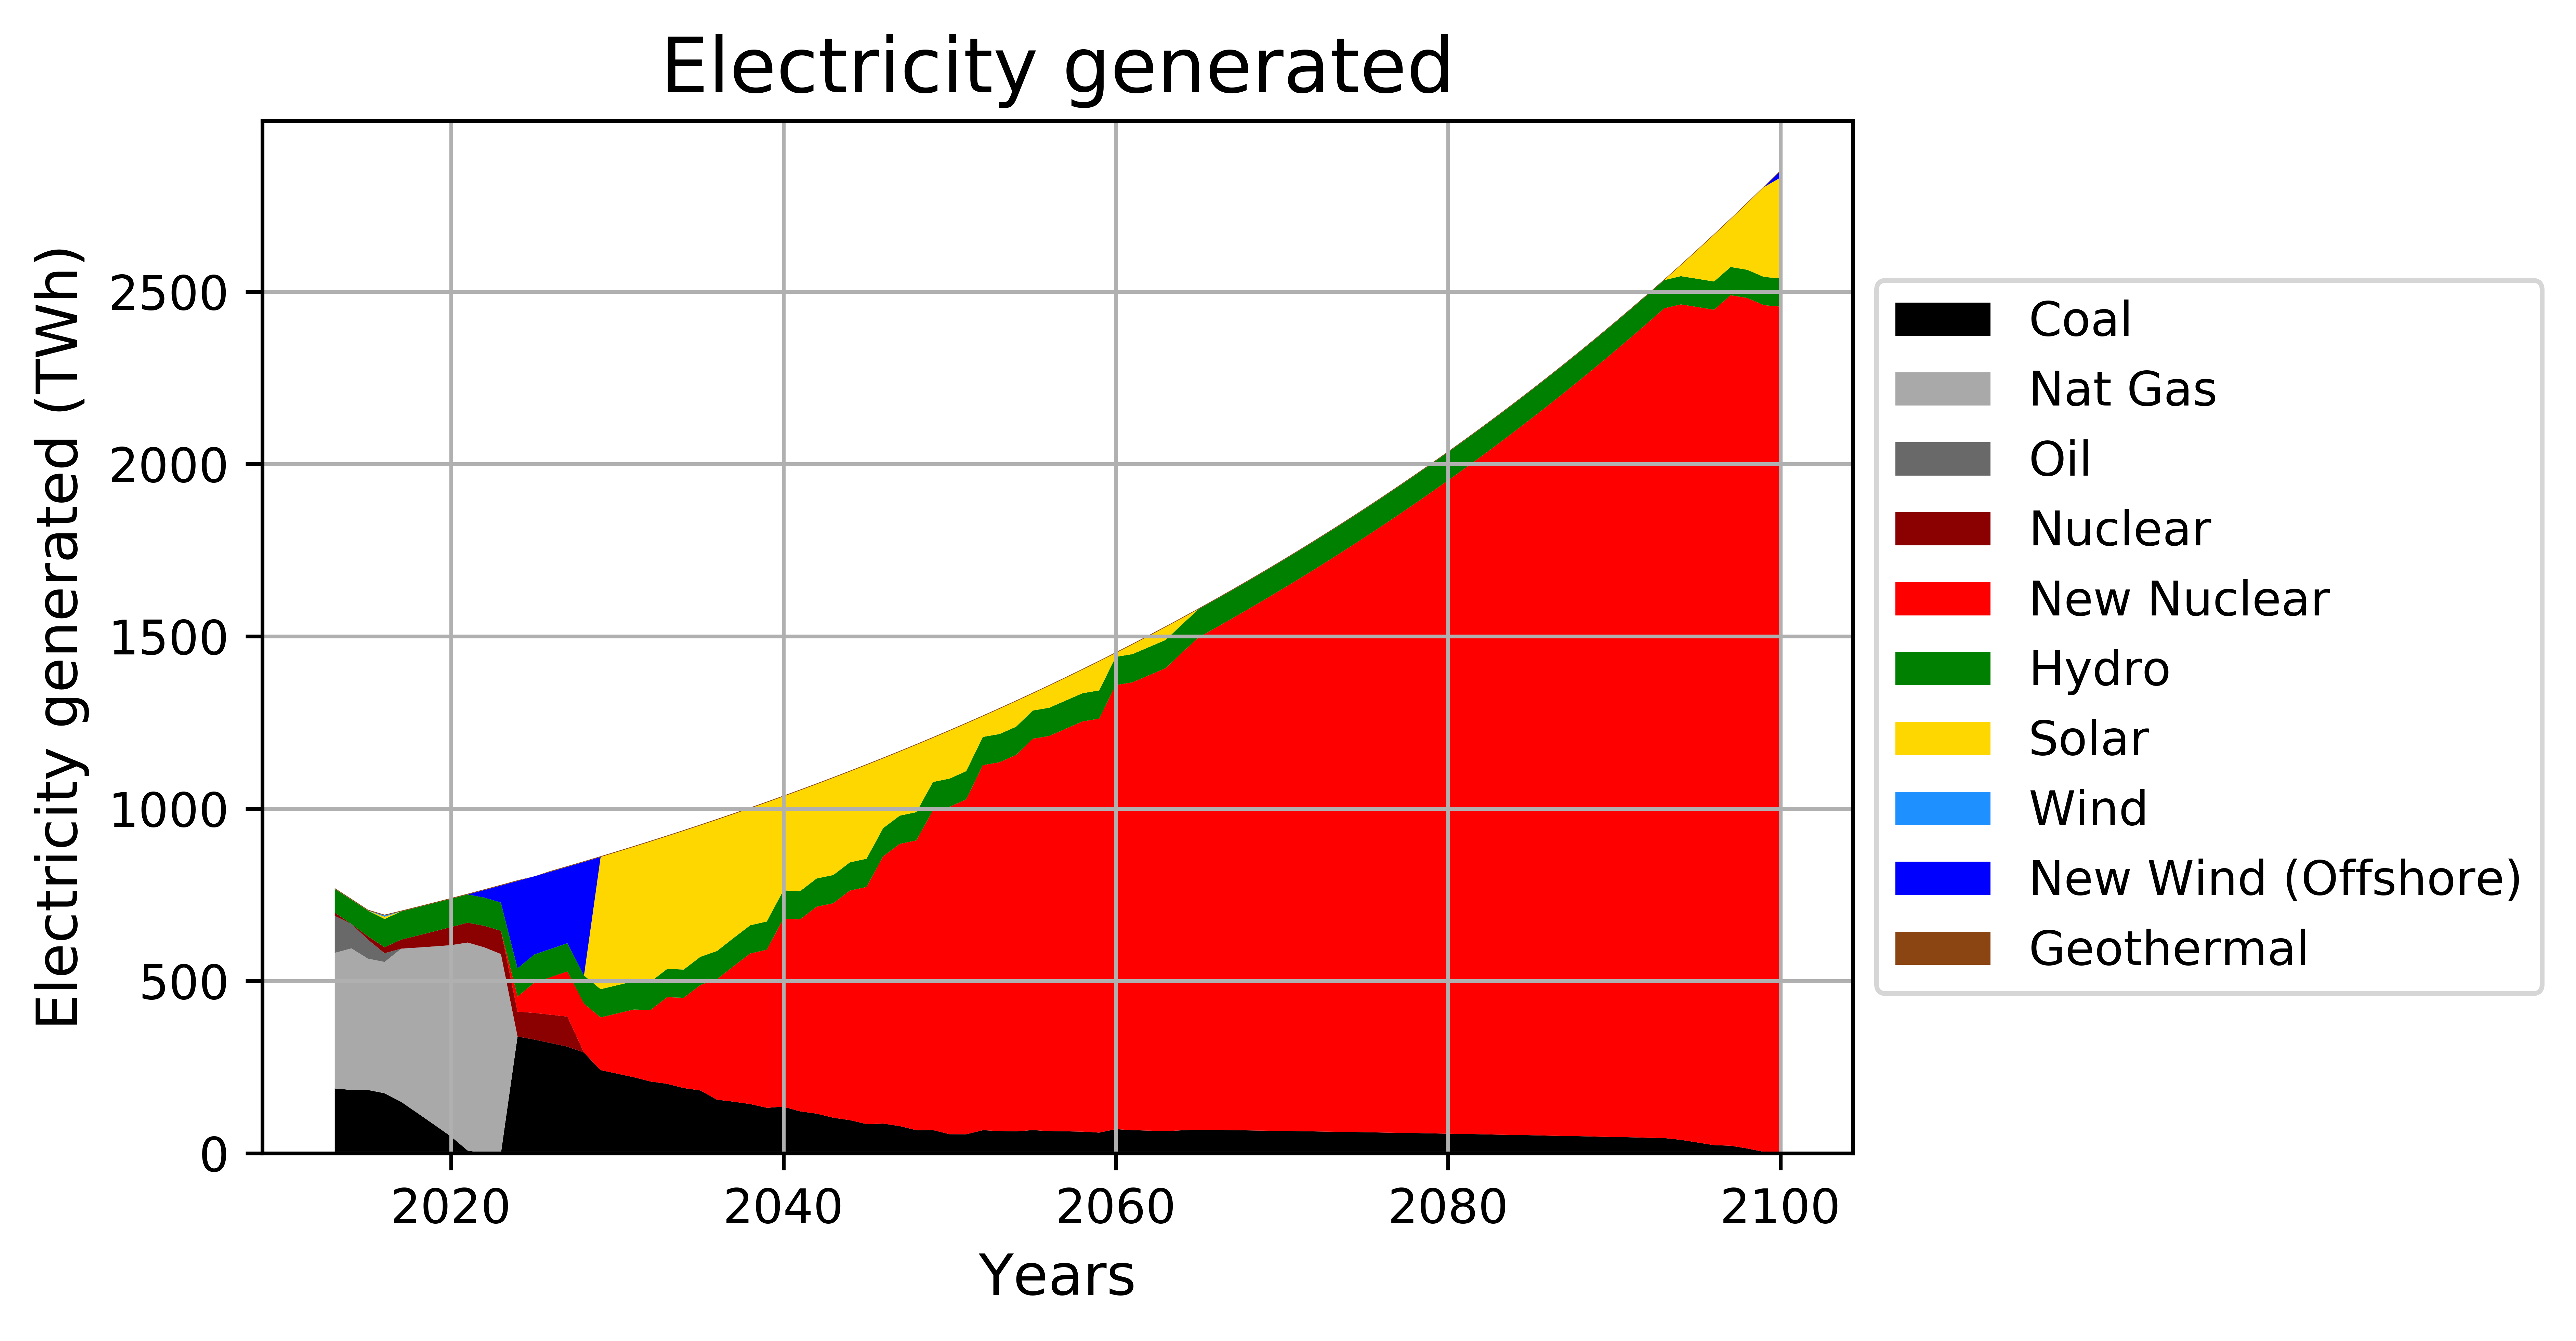
\includegraphics[scale=0.6]{./images/i2cner_nuc_elc}
    \end{center}
          \caption{Scenario 3 Electricity Generation.}
    \label{s3e}
  \end{figure}
\end{frame}

\begin{frame}
  \begin{figure}[htbp!]
    \begin{center}
      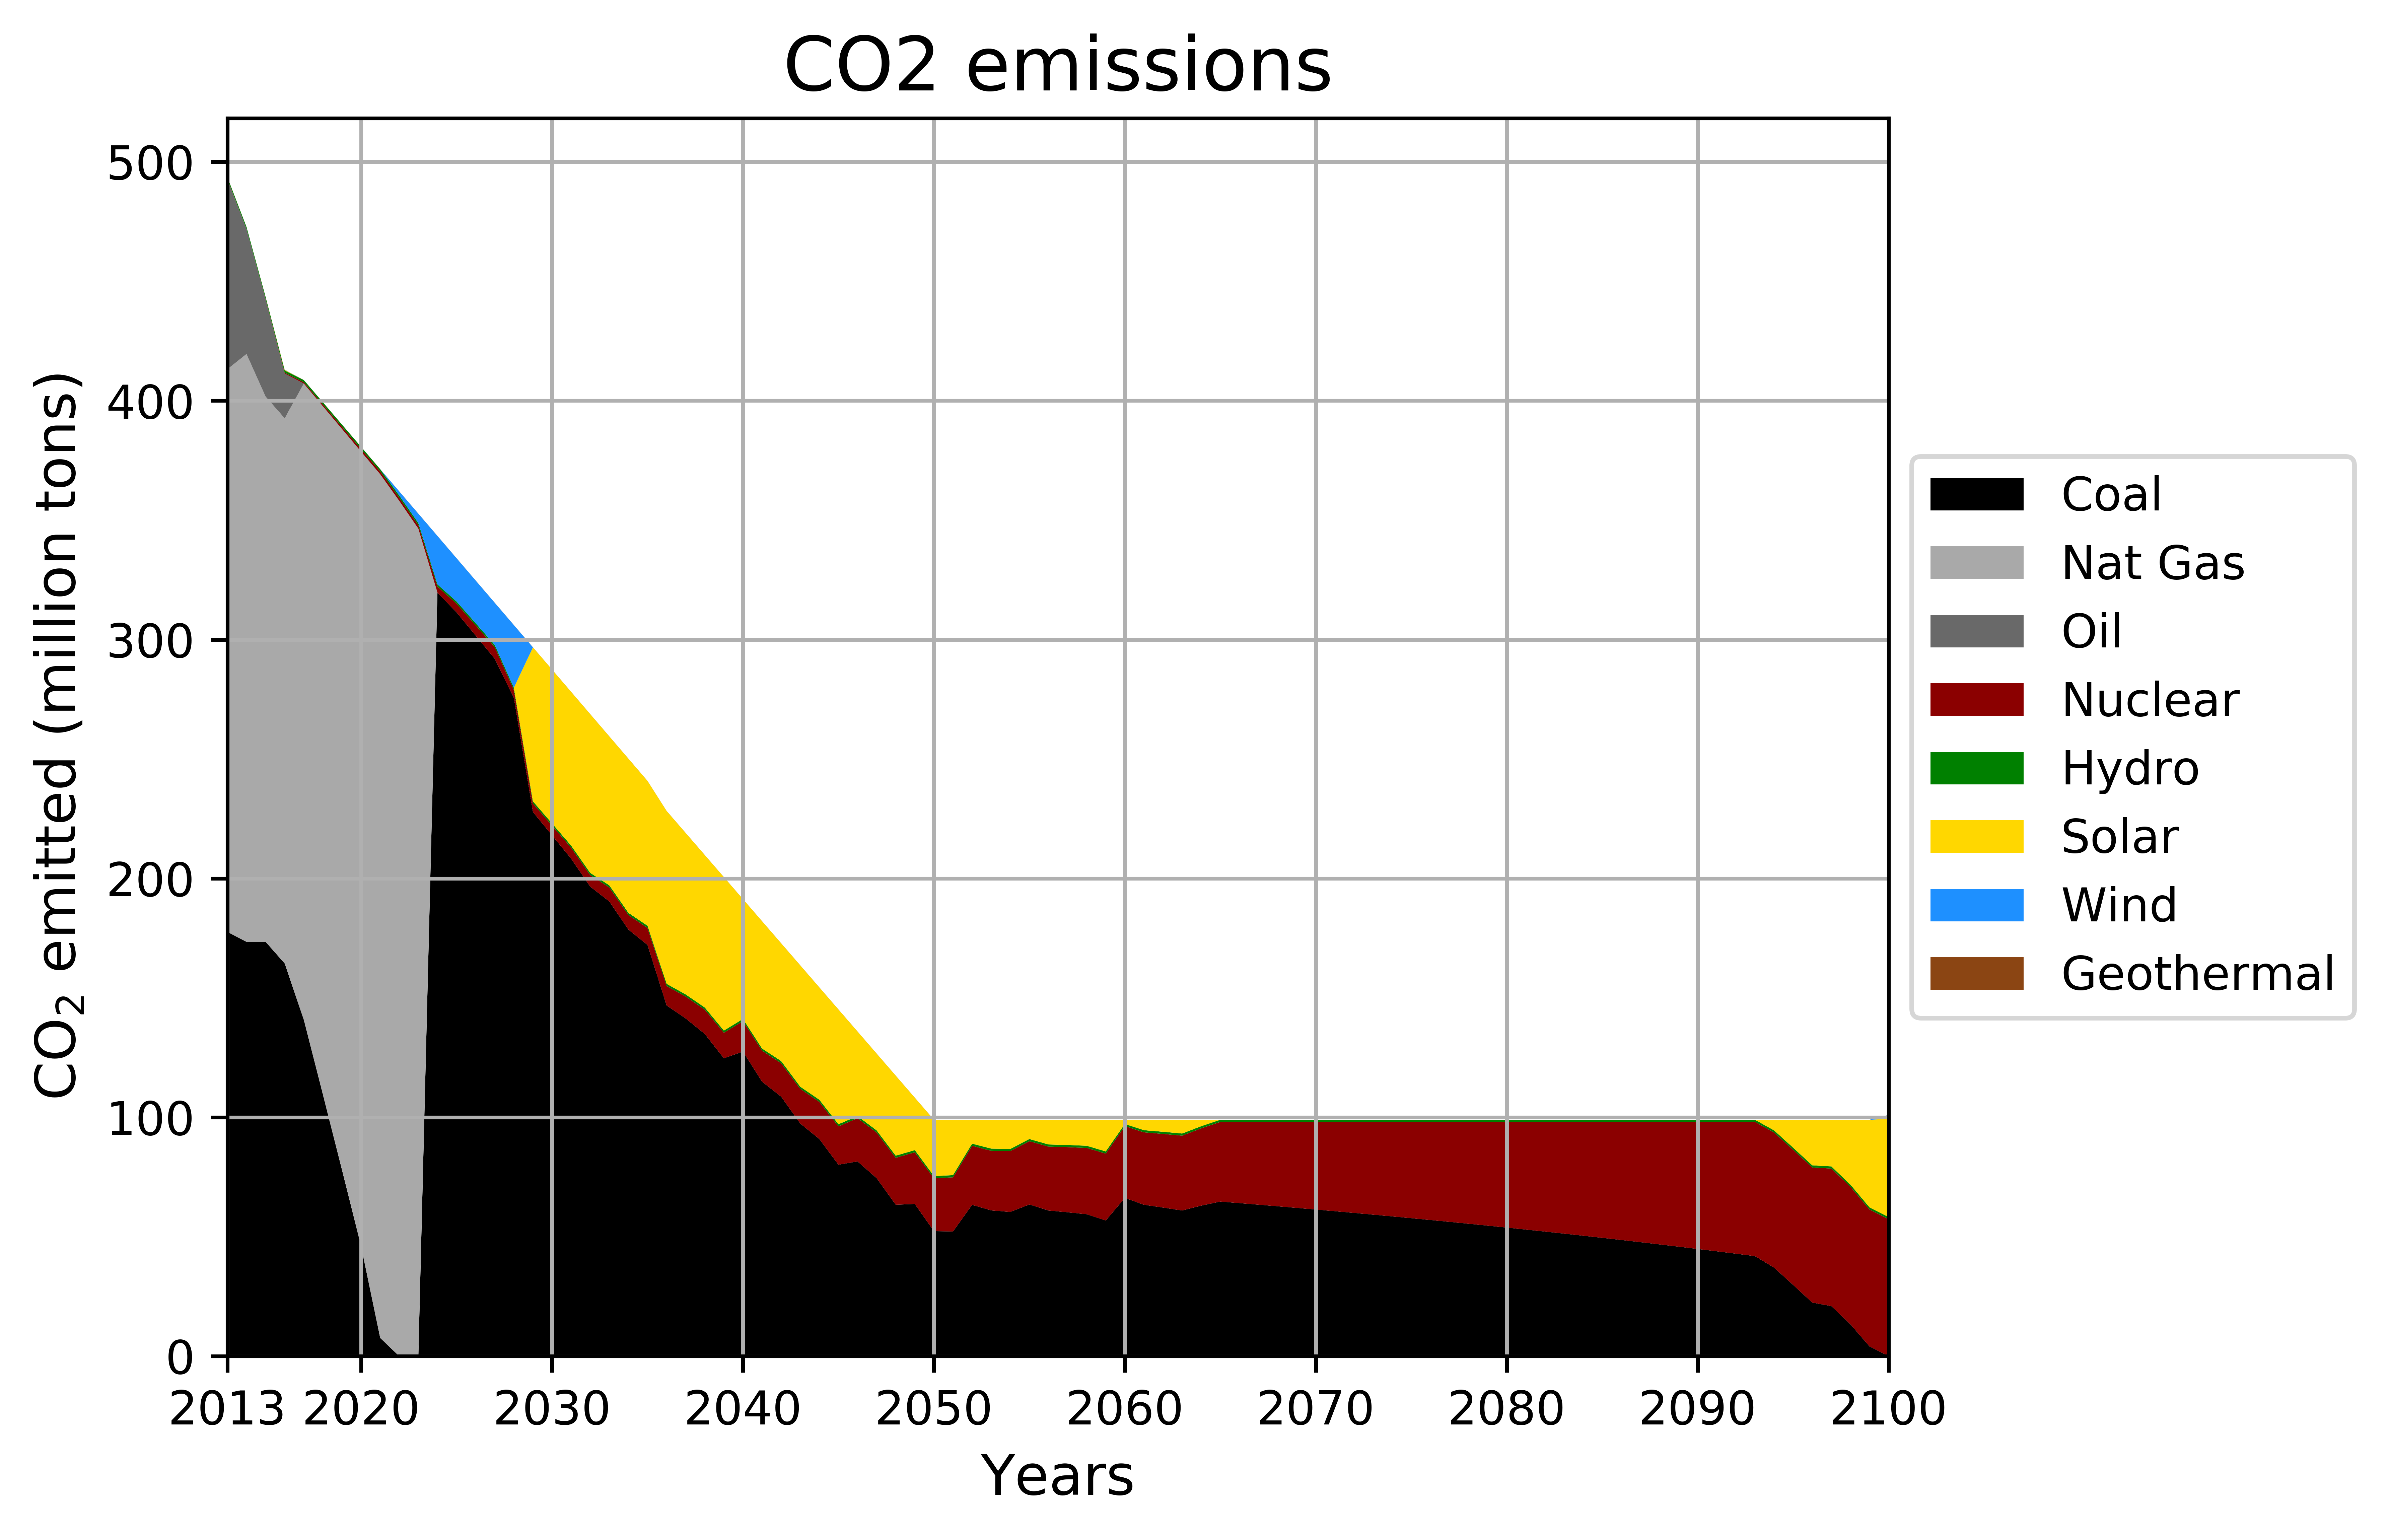
\includegraphics[scale=0.6]{./images/i2cner_nuc_co2}
    \end{center}
          \caption{Scenario 3 CO$_2$ emissions.}
    \label{s3c}
  \end{figure}

\end{frame}
\subsection{Scenario 4}
\begin{frame}
  \frametitle{Scenario 4: With I$^2$CNER technology, no new nuclear}
  % a comment
  \begin{figure}[htbp!]
    \begin{center}
      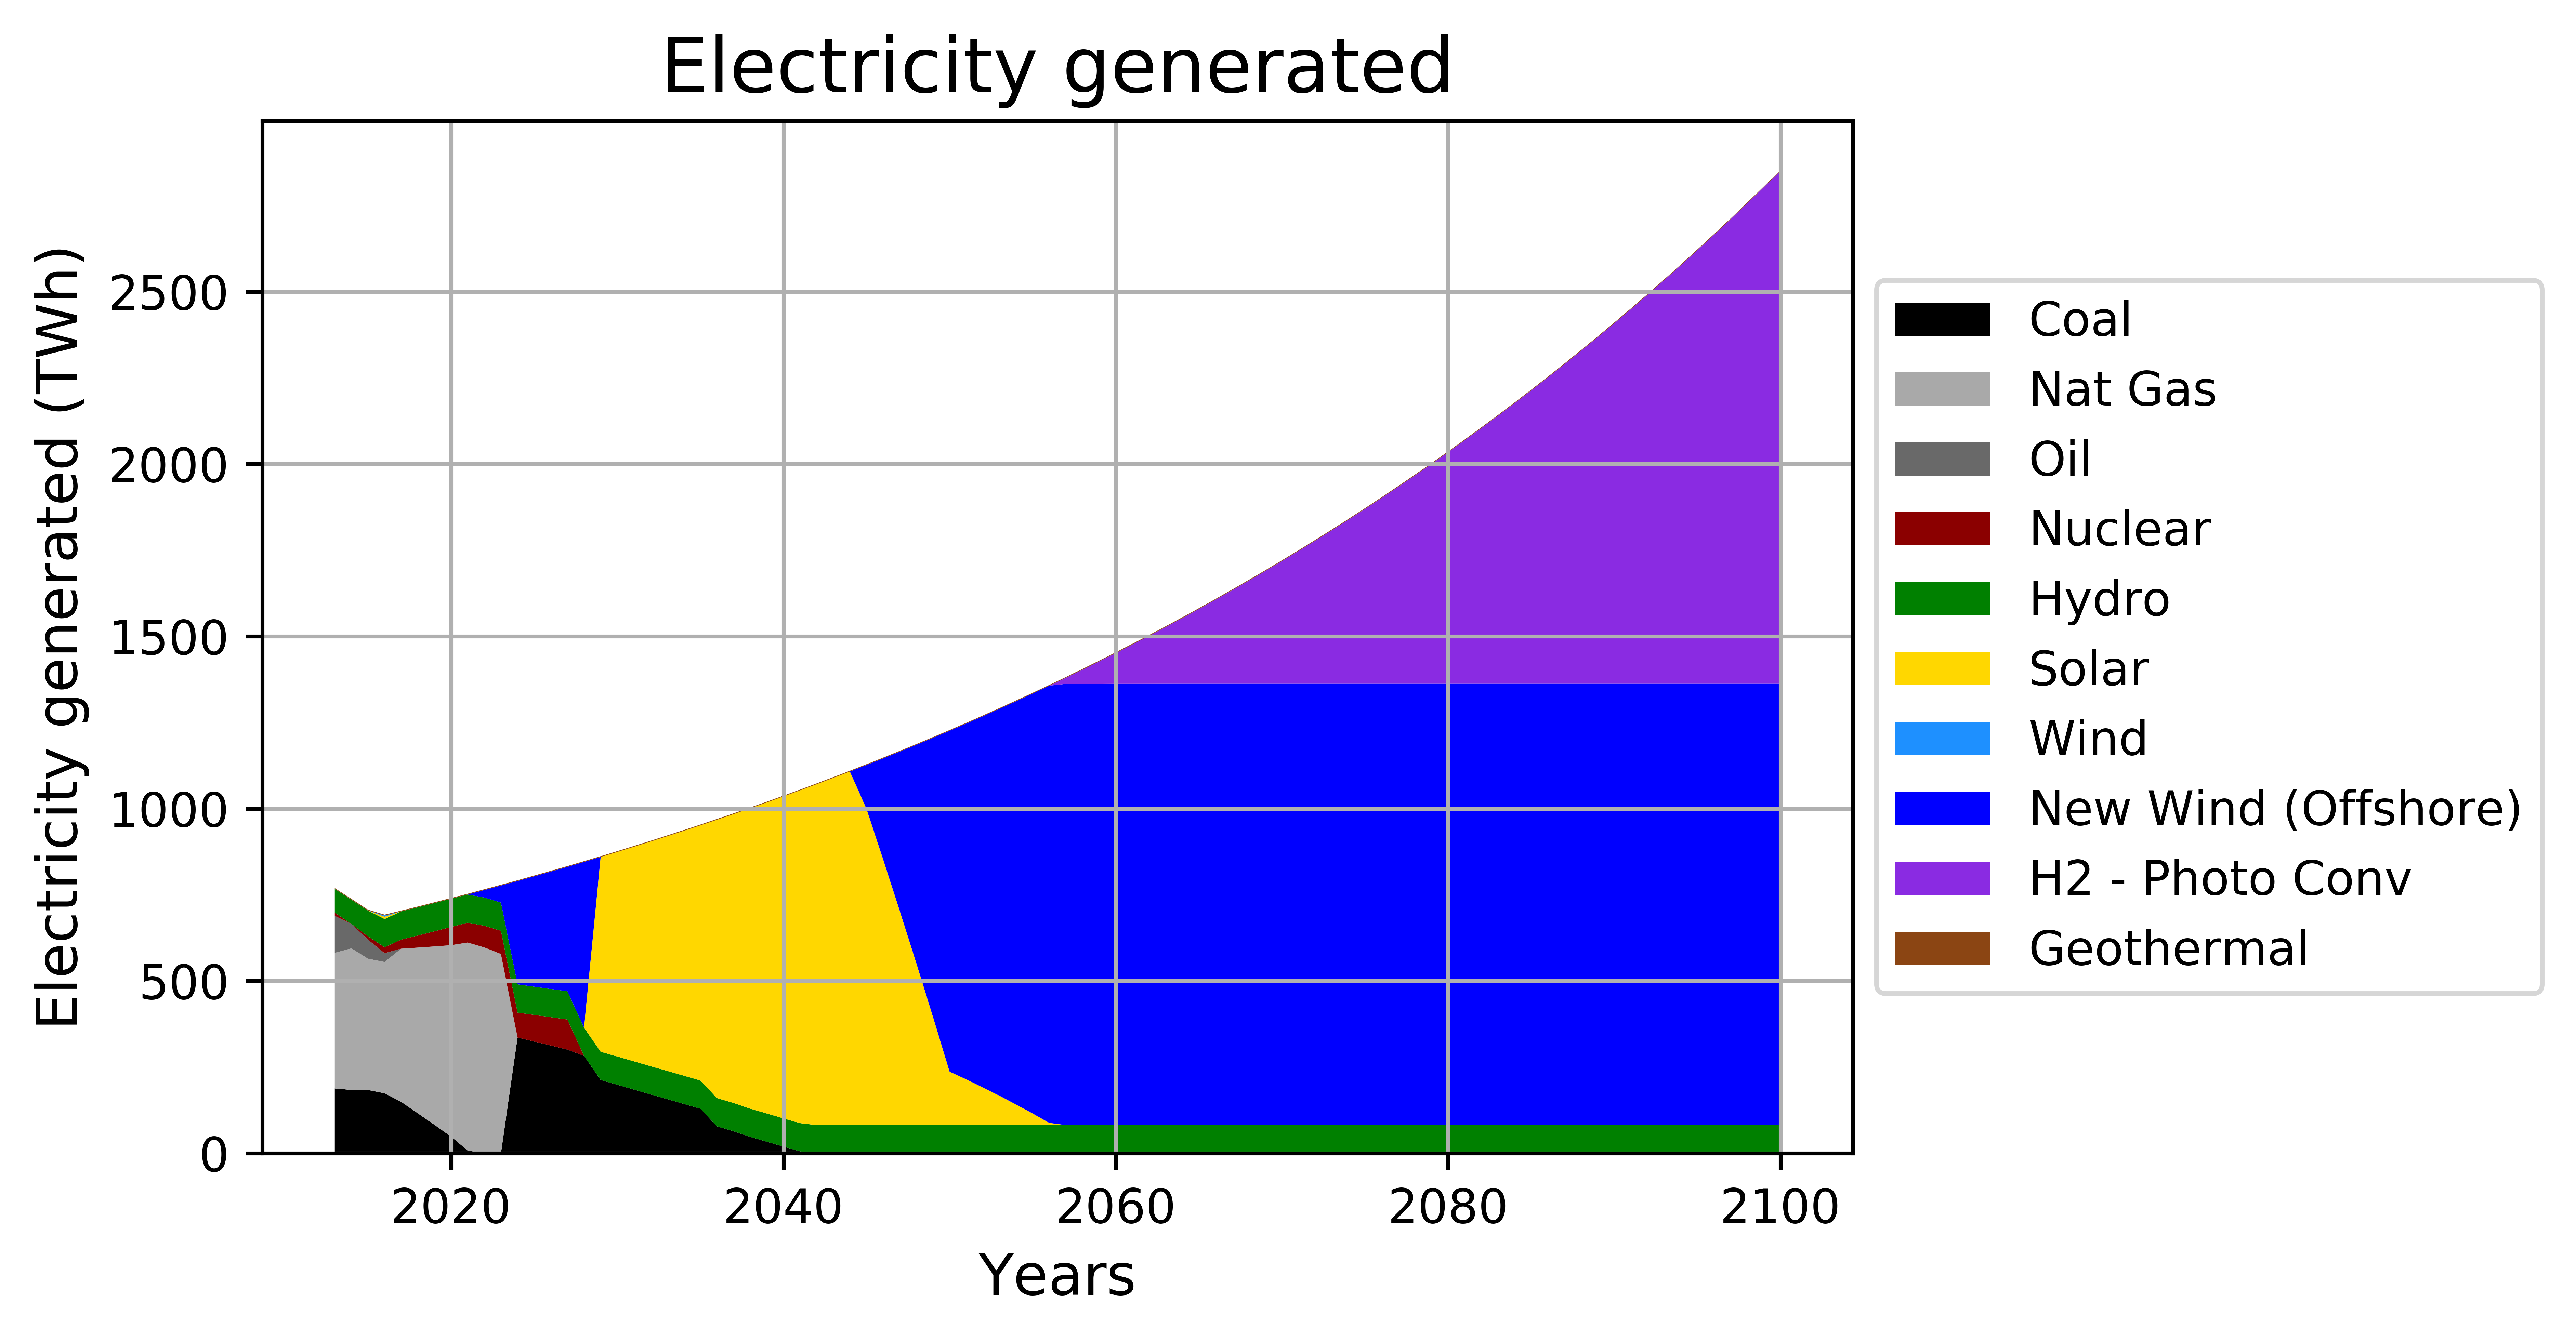
\includegraphics[scale=0.5]{./images/i2cner_nonuc_elc}
    \end{center}
          \caption{Scenario 4 Electricity Generation.}
    \label{s4e}
  \end{figure}
\end{frame}

\begin{frame}
  \frametitle{Scenario 4: With I$^2$CNER technology, no new nuclear}
  \begin{figure}[htbp!]
    \begin{center}
      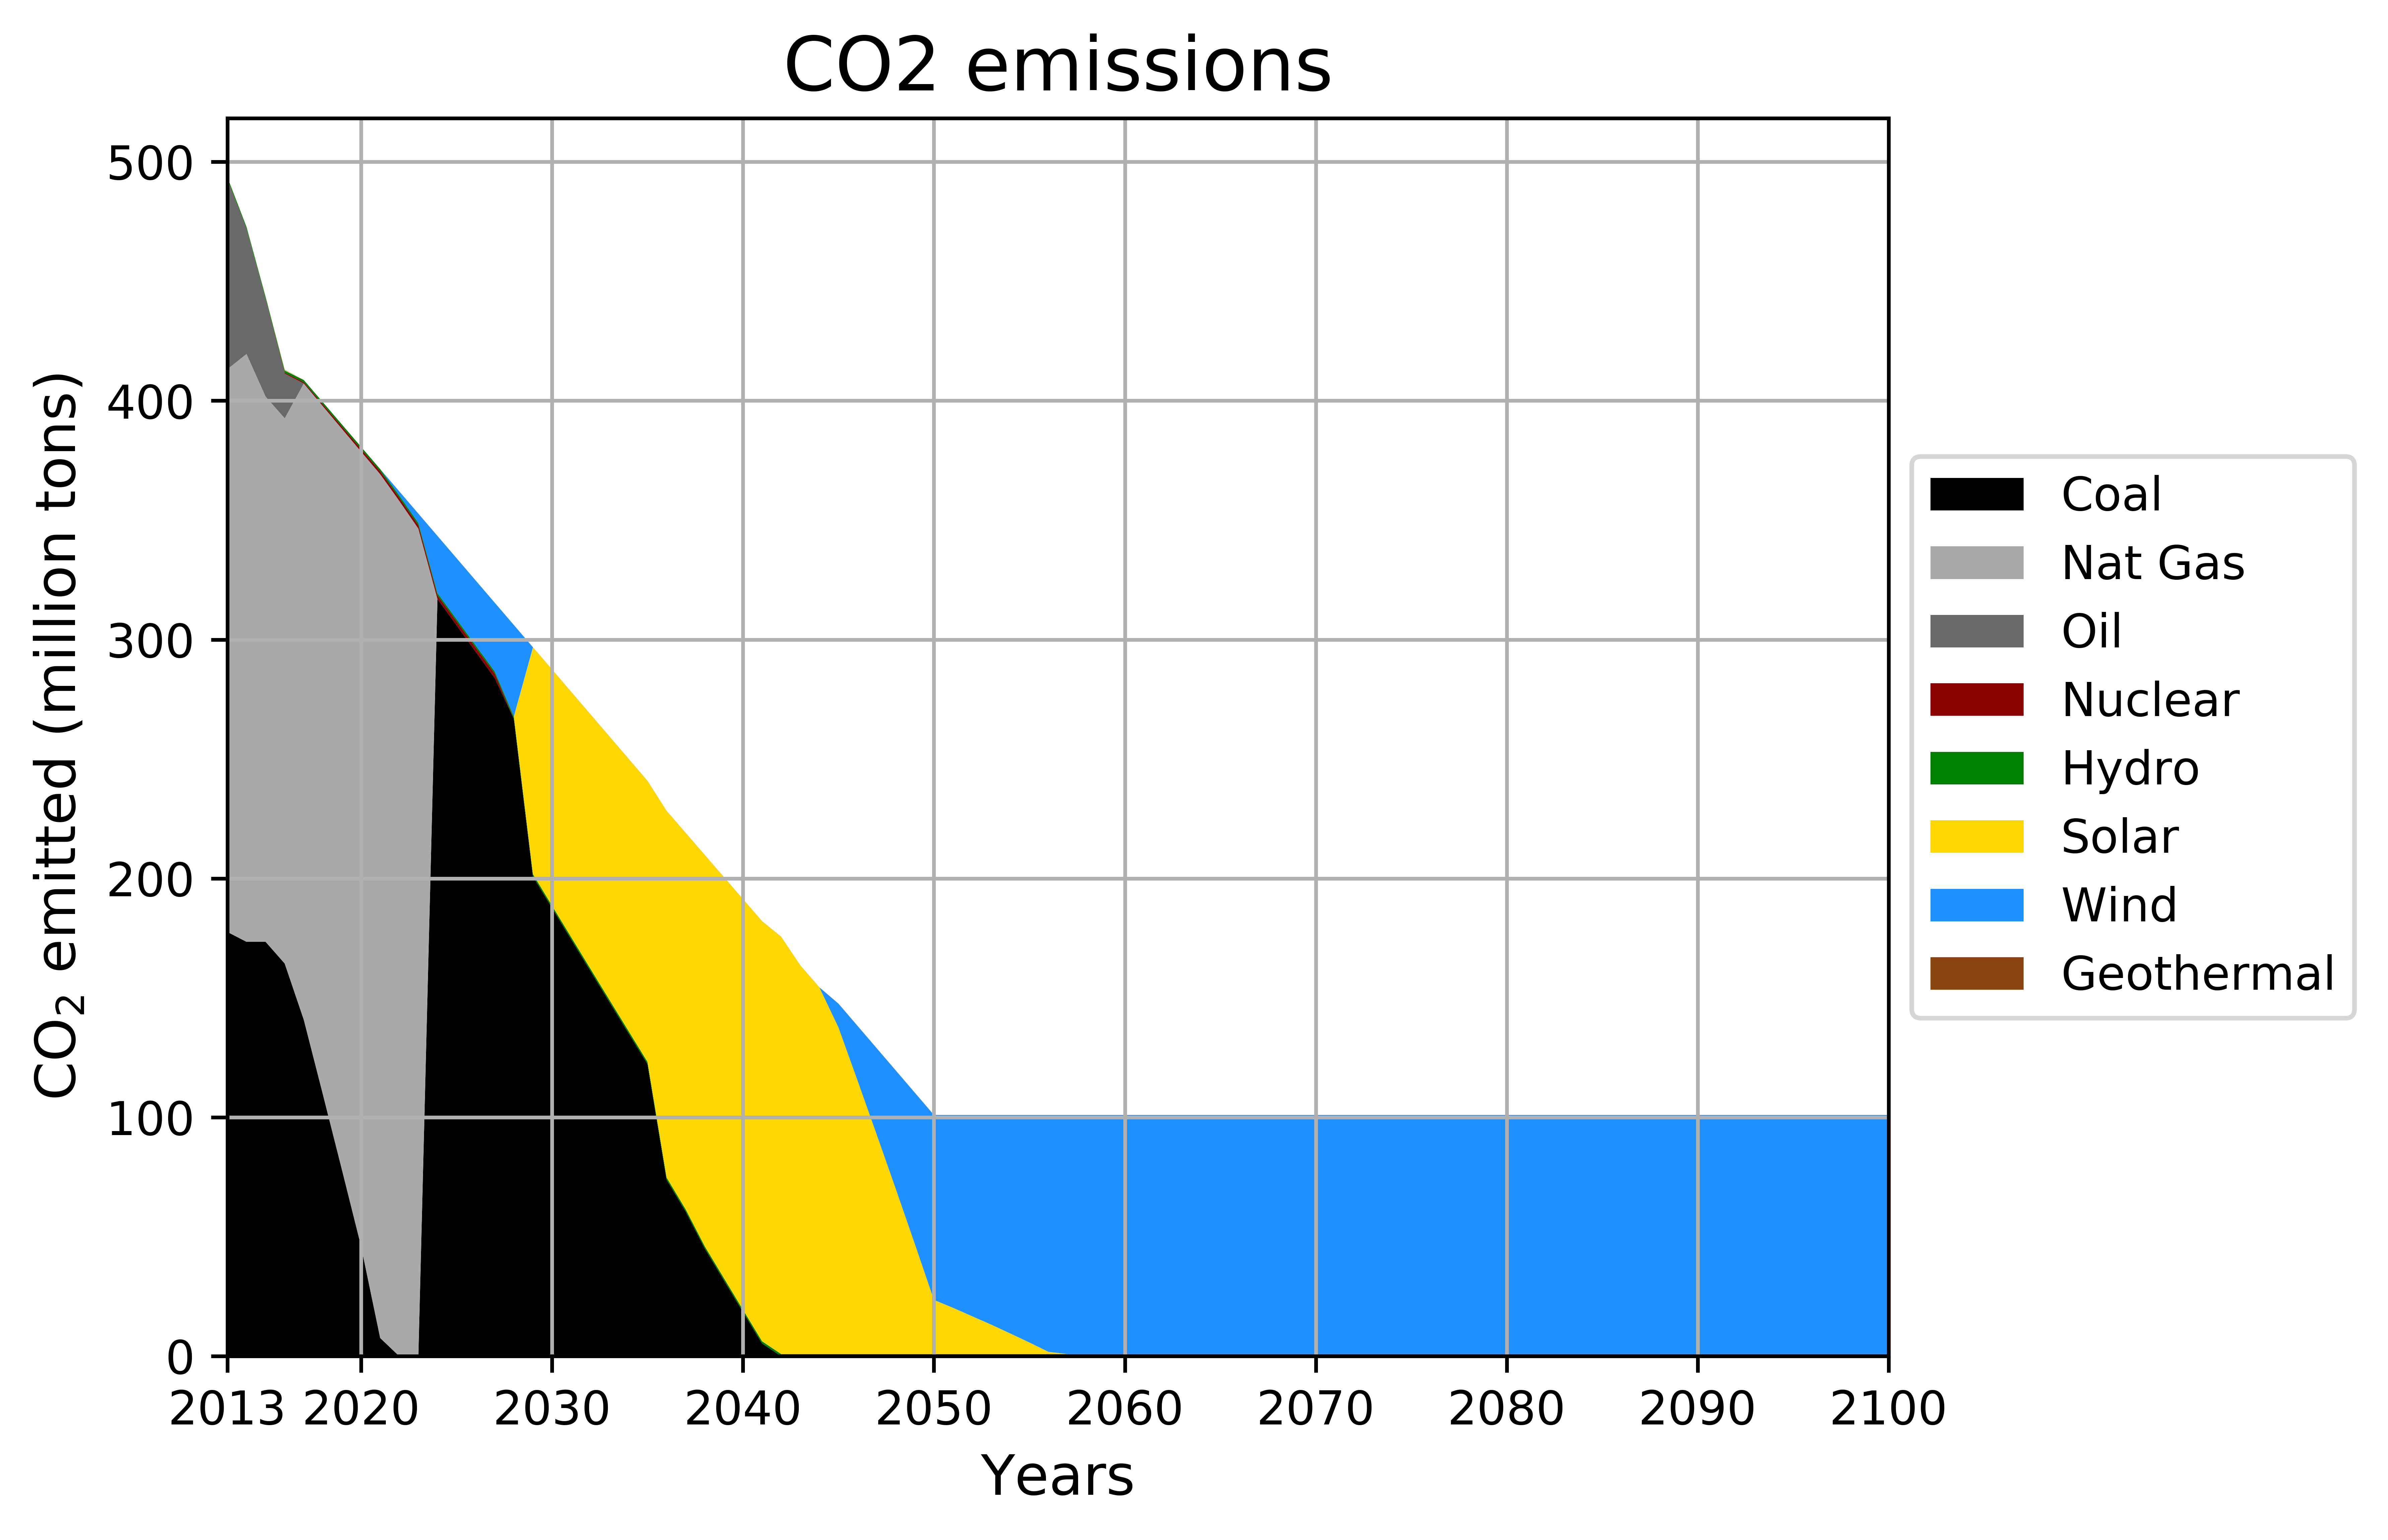
\includegraphics[scale=0.5]{./images/i2cner_nonuc_co2}
    \end{center}
          \caption{Scenario 4 CO$_2$ emissions.}
    \label{s4c}
  \end{figure}

\end{frame}
\section{Conclusion}
\begin{frame}
  \frametitle{Conclusion}
        We showed many things.
        \begin{itemize}
                \item Cats are peculiar
                \item Blue and Orange are fierce colors
                \item Math can be rendered nicely
                \item Cite your sources
        \end{itemize}
\end{frame}

\section{Future work}
\begin{frame}
  \frametitle{Future work}
   \begin{itemize}
   
   \item Transition from model creation to model refinement.
   
   \item Capture realistic, gradual transitions.
   
   \item Incorporate fluctuations in demand.
   
   \item Add energy storage to supplement renewables and H$_2$.
   
   \item Incorporate more I$^2$CNER technologies.
   
   \item Conduct sensitivity and cost analysis.
   
   \end{itemize}

\end{frame}
\section{Acknowledgments}

The author(s) gratefully acknowledge the support of the International Institute for Carbon Neutral Energy Research (WPI-I2CNER), sponsored by the Japanese Ministry of Education, Culture, Sports, Science and Technology. We are also grateful to Kenshi Itaoka and Hadi Farabi-Asl for providing valuable discussions related to this project, and to Gavin Davis and Nataly Panczyk for editing drafts.

The authors contributed to this work as described below.

Anshuman Chaube designed simulation models, conducted sensitivity analysis, and wrote the original draft of the paper.

Andrew Chapman conceived and contributed to conception of the simulations, designed simulation models, and wrote the original draft of the paper. 

Akari Minami translated data from Japanese to English, and assisted with testing and performing simulations.

James Stubbins supervised the work, conceived and contributed to conception of the simulations, and reviewed drafts of the paper.

Kathryn D. Huff supervised the work, conceived and contributed to conception of the simulations, and reviewed drafts of the paper.  Prof. Huff is supported by the Nuclear Regulatory Commission Faculty Development Program, the National Center for Supercomputing Applications, the International Institute for Carbon Neutral Energy Research (WPI-I2CNER), sponsored by the Japanese Ministry of Education, Culture, Sports, Science and Technology, and  DOE ARPA-E MEITNER program award DE-AR0000983.

%%--------------------------------%%
%%--------------------------------%%
\begin{frame}[allowframebreaks]
  \frametitle{References}
  \footnotesize \bibliographystyle{ieeetr}
  { \bibliography{2019-chaube-i2cner-poster} }

\end{frame}

%%--------------------------------%%


\end{document}



